\begin{appendix}
\section{Matsubara Frequencies and Fast Fourier Transform}
In order to solve the impurity model we have to perform several Fourier Transforms.
As we consider electrons, the Green's function in imaginary time is antiperiodic by shifts of $\beta$, so we have to use fermionic Matsubara frequencies $ω_n:=π(2n+1)/β$.
The Fourier Transformations are given by (no more implicit $\beta$):

\begin{equation}
  G(i ω_n) := \int\limits_0^β \mathrm{d}τ G(τ) e^{i ω_n τ} ,
  \quad
  G(τ) = \frac{1}{β} \sum_{i ω_n} G(i ω_n) e^{-i ω_n τ}
\end{equation}
%
For efficient calculations we use the FFT-algorithm of the numpy package. Therefore we have to adapt our definitions to the implementation of the numpy library. The numpy library calculates its Fourier Transform by:
\begin{equation}
  A_k = \mathrm{FFT}(a_m) =  \sum_{m=0}^{n-1} a_m \exp\left\{-2\pi i{mk \over n}\right\}
   \qquad k = 0,\ldots,n-1.
\end{equation}
Hence, we discretize the Matsubara Fourier transformation
\begin{align}
  G(i ω_{-n}) &\approx \sum_{k=0}^{N-1} \Delta τ \, G(\Delta τ \, k) \exp{\left(i \frac{π (-2n+1)k}{N}\right)}\\
          &=\frac{\beta}{N} \sum_{k=o}^{N-1} \left( G(\Delta τ \, k)\exp{\left(i π \frac{k}{N}\right)}  \right)  \exp{\left(i \frac{-2 π n k}{N}\right)}\\
	  &= \frac{\beta}{N} \mathrm{FFT}\left( G(\Delta τ \, k)\exp{\left(i π \frac{k}{N}\right)}\right), \label{eq:MFFT}
\end{align}
where $\Delta τ = \frac{\beta}{N}$.
The same can be carried out for the inverse Fourier Tranforms:
\begin{align}
	G(\Delta τ k) &= \frac{N}{β} e^{-i π \frac{k}{N}}\frac{1}{N}\sum_{ω_n}G(i ω_{-n}) e^{i 2π n k/N}\\
	&= \frac{N}{β} e^{-i π \frac{k}{N}}\mathrm{IFFT}(G(iω_{-n})) \label{eq:IMFFT}.
\end{align}
\begin{figure}[h]
	\centering
	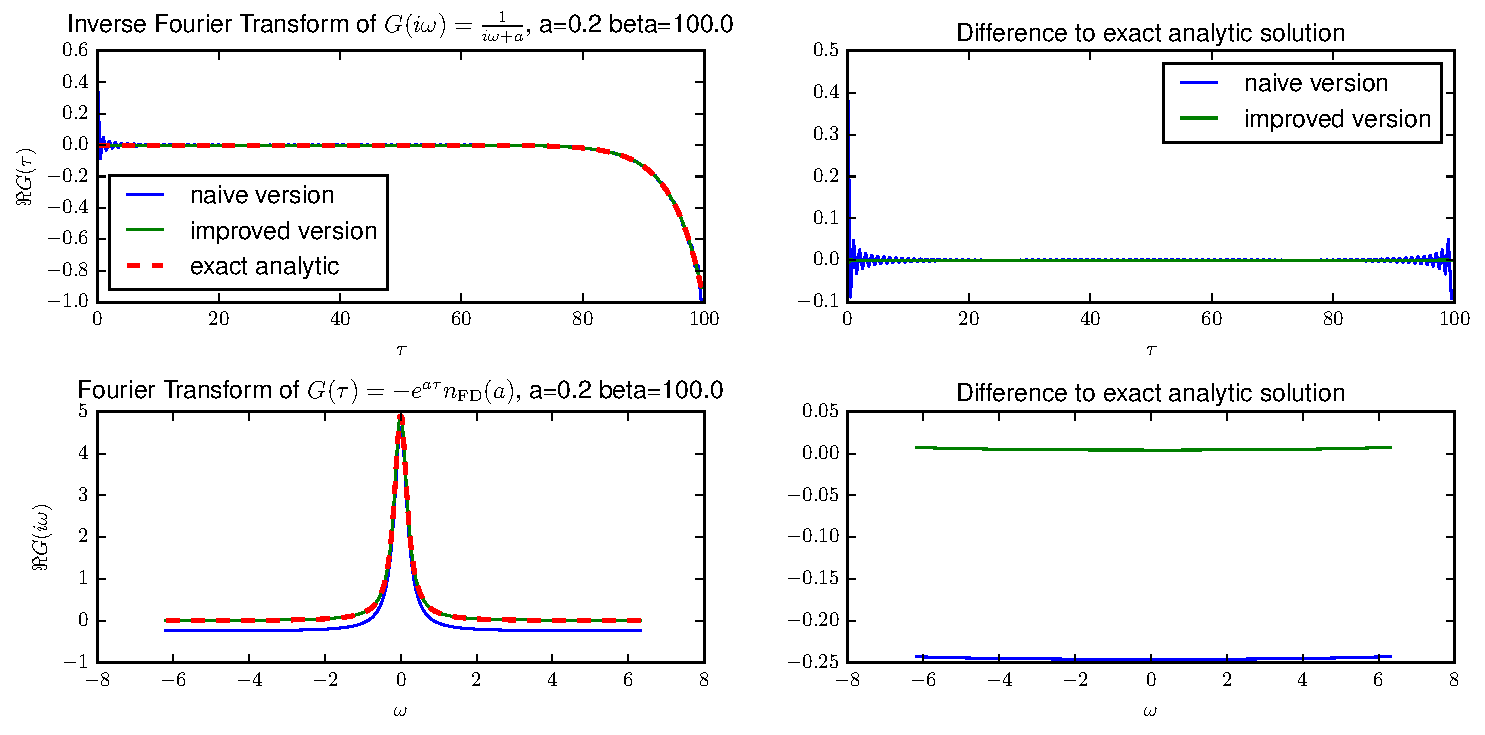
\includegraphics[width=\textwidth]{Matsubara_Fourier_fig}
	\caption{Comparison of the different discretized Fourier Transforms. The improved version, by manually transforming the $1/i \omega$ part, approximates the exact transformation significantly better. }
	\label{fig:fourier_traf}
\end{figure}

Unfortunately the ``naive'' implementations \eqref{eq:MFFT} and \eqref{eq:IMFFT} cause numerical problems, since according to \eqref{G_largefreq} Green's functions only decay as $1/ i\omega_n$ in frequency space. As the frequency sum is cut off by the finite number of points used, one can strongly increase the accuracy by manually transforming the $1/ i\omega_n$ part. By contour integration, it is shown that ($\tau \neq 0$)
%
\begin{align}
G(i\omega_n) = \frac{1}{i\omega + a}
\quad &\Leftrightarrow \quad
G(\tau) = \Theta(\tau) \frac{- e^{a \tau}}{e^{\beta a}+1} + \Theta(-\tau) \frac{e^{a \tau}}{e^{-\beta a}+1} 
\\
	G(i ω_n) =\frac{1}{i ω_n} \quad &⇔ \quad G(τ)=-\frac{1}{2} + \Theta(-\tau)
	\label{eq:ff_pair}
\, .
\end{align}
Consequently the improved version of our Fourier transformation for $τ∈[0,β)$ is given by subtracting and adding the relevant terms before and after the transformation.
\begin{align}
	G(i ω_{-n})&= \frac{1}{i ω_{-n}}+\frac{\beta}{N} \mathrm{FFT}\left( \left(G(\Delta τ \, k)+\frac{1}{2}\right)\exp{\left(i π \frac{k}{N}\right)}\right)\\
	G(\Delta τ k)&= -\frac{1}{2}+\frac{N}{β} e^{-i π \frac{k}{N}}\mathrm{IFFT}\left(G(iω_{-n})-\frac{1}{i ω_{-n}}\right)
	\label{eq:improved_fft}
\end{align}
The improvement can be seen in \figref{fig:fourier_traf}, where we compare the exact Fourier transformation of $G(i ω)=\frac{1}{iω+a}$ to our discretized versions. The naive version shows significant deviations to the analytic solution, whereas our improved version approximates the exact one very well.  


\section{Analytic continuation}
\begin{figure}[htb]
  \begin{center}
    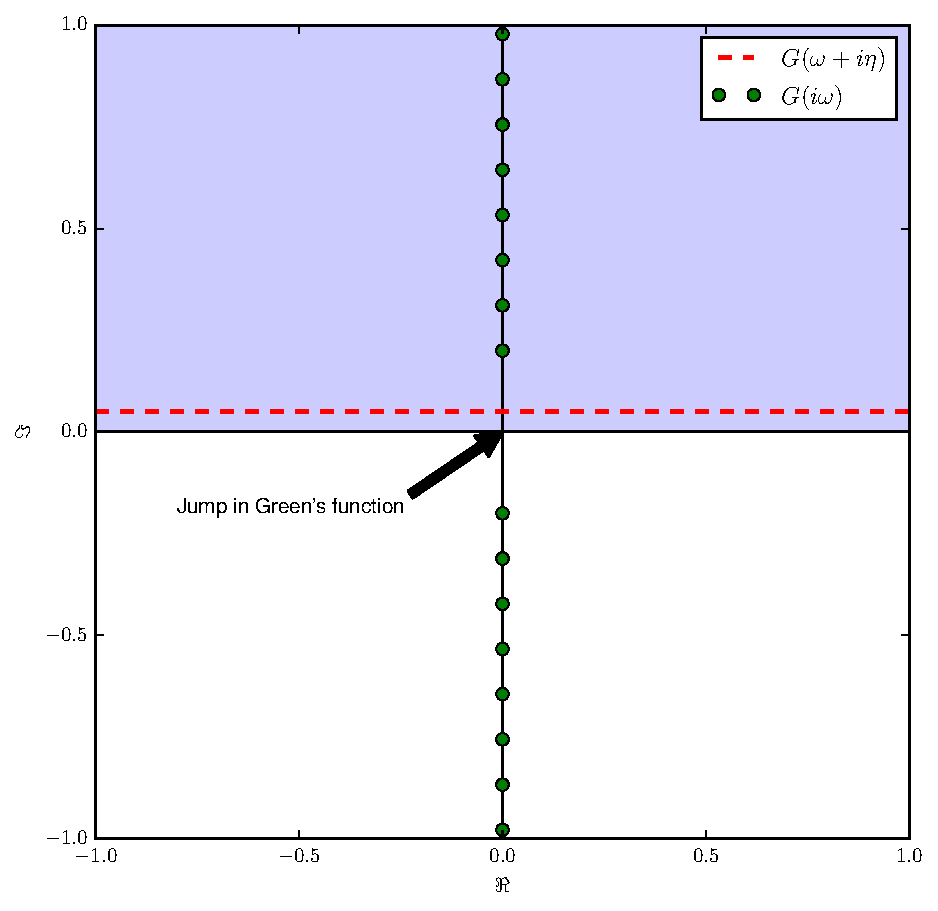
\includegraphics[width=0.7\textwidth]{analytic_continuation}
  \end{center}
  \caption{As the retarded Green's function (red) lies slightly above the real axis and the Matsubara Green's function shows discontinuous jumps at zero frequency, we only take the positive frequencies to calculate the Padé approximation. Assuming that the Green's function is analytic in the upper half plane (blue), we expect the analytic continuation with the rational function to approximate the retarded Green's function both for positive and negative frequencies. }
  \label{fig:analytic_continuation}
\end{figure}


In order to calculate the spectral function $\mathcal{A}$, we have to perform the analytic continuation of the Matsubara Green's function.
This is a hard problem as we need the functional dependence of $G(iω_n)$ and the only information available is given by discrete points on the imaginary axis.
The central idea is now to interpolate our discrete points by a rational function, called Padé approximation, and use this function to do the analytic continuation. 
An efficient algorithm to calculate the Padé approximation can be found in \cite{padepaper}. However, as the Padé approximation is continuous, whereas the Green's function exhibits non-continuous jumps, we have to think about, which values to use for the interpolation.

In the results of the DMFT-loop we observed discontinuous jumps in the Matsubara Green's function at zero frequency.
As we expect the Greens function to behave non-analytically only on the real axis, we can restrict ourselves to the positive or to the negative frequencies in order to calculate the interpolation and use the symmetry of the Green's function $G(iω)=G(-iω)^*$ to get its values on the opposite half plane.

Since the retarded Green's function is given by $G(i ω \to ω + i 0^+)$ lies slightly above the real axis, we can use the positive frequencies on the imaginary axis to calculate the interpolation and perform the analytic continuation both for positive and negative frequencies of the retarded Green's function as can be seen in \figref{fig:analytic_continuation}.

Furthermore, we reduced the number of values to calculate the interpolation. In some cases this proved to be more stable, which is no surprise, as interpolation polynomials of high degree often show rapid oscillations.


\end{appendix}
